\documentclass[11pt]{article}

\usepackage[margin=1in]{geometry}
\usepackage[T1]{fontenc}
\usepackage[utf8]{inputenc}
\usepackage{lmodern}
\usepackage{microtype}
\usepackage{amsmath,amssymb,amsthm,mathtools}
\usepackage{bm}
\usepackage{booktabs}
\usepackage{longtable}
\usepackage{array}
\usepackage{multirow}
\usepackage{graphicx}
\usepackage{float}
\usepackage{caption}
\usepackage{subcaption}
\usepackage{enumitem}
\usepackage{hyperref}
\usepackage{xcolor}
\usepackage{listings}
\usepackage[ruled,vlined,linesnumbered]{algorithm2e}
\usepackage{siunitx}

\hypersetup{
  colorlinks=true,
  linkcolor=blue!50!black,
  citecolor=blue!50!black,
  urlcolor=blue!50!black,
  pdftitle={Runtime-Aware Characterization of Constrained QAOA Portfolio Optimization},
  pdfauthor={Author Name}
}

\renewcommand{\thesection}{\Roman{section}}
\renewcommand{\thesubsection}{\thesection.\Alph{subsection}}
\renewcommand{\thesubsubsection}{\thesubsection.\arabic{subsubsection}}

\newtheorem{lemma}{Lemma}
\newtheorem{proposition}{Proposition}
\newtheorem{theorem}{Theorem}

\lstdefinestyle{repo}{
  basicstyle=\ttfamily\small,
  numbers=left,
  numberstyle=\scriptsize\color{gray},
  keywordstyle=\color{blue!60!black},
  commentstyle=\color{green!40!black},
  stringstyle=\color{red!50!black},
  frame=single,
  breaklines=true,
  columns=fullflexible,
  keepspaces=true,
  showstringspaces=false
}
\lstset{style=repo}

\title{\textbf{Runtime-Aware Characterization of Constrained QAOA Portfolio Optimization:}\\
Classical Baselines, Mixer Architecture, and Hybrid-Loop Cost}
\author{Author Name\\
\small Overleaf-ready manuscript generated from committed repository evidence in \texttt{portfolio\_qaoa\_bench\_repo}}
\date{21 April 2026}

\begin{document}
\maketitle

\begin{abstract}
This manuscript studies constrained portfolio optimization with the Quantum Approximate Optimization Algorithm (QAOA) under a deliberately conservative, runtime-aware evaluation protocol. The underlying software artifact, \texttt{portfolio\_qaoa\_bench}, is not a single-instance demonstration but a characterisation platform that combines synthetic portfolio regimes, exact feasible references on small instances, a continuous-relaxation classical Markowitz baseline, constraint-preserving and penalty-based mixers, classical outer-loop optimizers, backend-aware circuit execution, and structured reporting. The core research question is operational rather than aspirational: when does a more sophisticated classical optimizer justify its runtime, shot, and queue overhead when tuning constrained QAOA?

The committed evidence yields three main findings. First, across the broad precomputed suite in \texttt{results/multi\_regime\_suite}, the classical Markowitz baseline achieves the best mean raw objective in all 26 study contexts and every reported Mann--Whitney comparison against Random Search in the aggregated artifact yields a corrected \(p\)-value of \(1.0\), indicating no statistically significant superiority of the quantum outer-loop optimizers over Random Search in that suite. Second, the dedicated mixer pilot in \texttt{results/mixer\_dominance\_pilot\_v2} shows that the \(\mathrm{XY}\) mixer is usually the stronger quantum design choice: it wins 17 of 24 quantum-only paired comparisons, whereas \(\mathrm{product}\text{-}X\) wins only one. However, the same pilot does \emph{not} support the stronger universal claim that mixer choice dominates optimizer choice: the variance proxy attributed to optimizer choice is \(0.0285\), exceeding the mixer contribution \(0.0113\). Third, a live IBM hardware execution on \texttt{ibm\_fez} reproduces the exact feasible energy on a three-asset instance, but only with valid-shot ratios between \(0.5625\) and \(0.78125\), revealing substantial hardware-induced leakage from the budget-feasible subspace despite use of the \(\mathrm{XY}\) mixer.

The significance of these results is methodological. The repository supports reproducible and falsifiable claims about when constrained-QAOA design choices matter, and the strongest present conclusion is not a claim of quantum advantage but an evidence-backed delimitation of where such a claim is \emph{not yet} warranted. The manuscript therefore advances the project as a scientific characterisation study of constrained QAOA, not as a premature benchmark of putative quantum superiority.
\end{abstract}

\section{Introduction}

Cardinality-constrained portfolio selection is a natural testbed for near-term quantum optimization because it couples a familiar financial objective to a genuinely combinatorial feasible set. In its binary form, the decision variable \(x \in \{0,1\}^n\) encodes inclusion of \(n\) candidate assets subject to a fixed budget \(\sum_i x_i = B\), and the underlying optimization objective is a discrete Markowitz functional balancing risk and return \cite{markowitz1952portfolio,kochenberger2014qubo,lucas2014ising}. This structure is attractive for QAOA because it can be expressed as a quadratic unconstrained binary optimization (QUBO) instance and then embedded into an Ising Hamiltonian \cite{farhi2014qaoa,hadfield2019qaoa}. At the same time, the problem exposes the central weakness of many near-term quantum optimization papers: a small improvement in an energy proxy is often reported without a clear accounting of classical baselines, optimizer overhead, constraint handling, or hardware execution cost \cite{cerezo2021vqa,proctor2025benchmarking,nation2025benchpress}.

The present repository was built to address that weakness directly. Its guiding question is not whether QAOA can produce a plausible portfolio on a single synthetic instance, but rather whether increasingly sophisticated classical \emph{outer-loop} optimization is practically justified when the inner quantum loop is constrained, noisy, and costly. That question is scientifically sharper than the common ``which optimizer won on one problem?'' formulation because it explicitly separates three effects that are too often conflated: the physics of the ansatz, the geometry of the constrained objective, and the classical overhead required to exploit either of them.

The code base therefore implements four comparison points under shared evaluation plumbing: Random Search, SPSA, Bayesian Optimization (BO), and a classical Markowitz baseline. It also exposes two distinct QAOA philosophies. The \(\mathrm{XY}\) mixer with Dicke-state initialization encodes the budget constraint into the circuit itself, whereas the \(\mathrm{product}\text{-}X\) mixer delegates feasibility to a QUBO penalty in the objective. This distinction is not cosmetic. It changes the reachable subspace, the two-qubit gate count, the interaction with noise, and the interpretation of optimizer trajectories \cite{hadfield2019qaoa,fuchs2022constrainedmixers,he2023alignment,kordonowy2026lie}.

The experimental evidence committed in the repository supports an honest and non-trivial thesis. The strongest result is \emph{negative}: in the broad suite, the classical Markowitz baseline dominates every study slice stored in the precomputed artifact. The strongest positive quantum result is narrower: in the dedicated mixer pilot, the \(\mathrm{XY}\) mixer is usually better than the penalty-based \(\mathrm{product}\text{-}X\) mixer, but the pilot does not support the stronger universal claim that mixer choice dominates optimizer choice. The live hardware run on IBM's \texttt{ibm\_fez} backend closes the loop by showing that even on a tiny instance where the exact feasible energy is recovered, hardware noise materially reduces feasible-shot occupancy.

The main contributions of this manuscript are as follows.
\begin{itemize}[leftmargin=1.5em]
\item It formalizes the repository as a reproducible characterisation study for constrained QAOA portfolio optimization rather than a score-only benchmark.
\item It derives the exact QUBO, feasible-subspace, and mixer-preservation mathematics used by the implementation.
\item It documents the software architecture, optimizer design, runtime accounting, and noise-model proxies used in the committed code.
\item It reports the committed broad-suite, mixer-pilot, and live-IBM results with explicit numerical citations to tables, figures, and listings.
\item It interprets the null findings and mixed findings as substantive scientific outcomes rather than as inconveniences to be hidden.
\end{itemize}

The remainder of the manuscript is structured as follows. Section~\ref{sec:background} situates the work within QAOA, constrained mixers, quantum finance, and benchmarking literature. Section~\ref{sec:theory} derives the mathematical model. Section~\ref{sec:methodology} describes the experimental system design. Section~\ref{sec:implementation} anchors the design in the repository code. Section~\ref{sec:experimental} documents the software and hardware setup. Section~\ref{sec:results} presents the empirical findings. Section~\ref{sec:discussion} interprets those findings and their limitations. Sections~\ref{sec:future} and~\ref{sec:conclusion} conclude. Appendices provide notation, environment details, extended tables, and code listings.

\section{Background and Related Work}\label{sec:background}

\subsection{QAOA, constrained mixers, and trainability}

QAOA alternates evolution under a problem Hamiltonian and a mixing Hamiltonian, with classical optimization over the corresponding angles \cite{farhi2014qaoa}. Its broader generalization, the Quantum Alternating Operator Ansatz, explicitly accommodates constrained combinatorial problems by allowing nonstandard mixers and initialization rules tailored to the feasible set \cite{hadfield2019qaoa}. This generalization is central here because portfolio selection with a hard budget constraint is precisely the sort of problem for which naive \(\sum_i X_i\) mixing may be algorithmically misaligned.

The modern literature on constrained QAOA has increasingly emphasized that the mixer is not a mere implementation detail. Fuchs \emph{et al.} formalize constrained mixers that preserve hard constraints throughout the evolution \cite{fuchs2022constrainedmixers}. He \emph{et al.} show, specifically for constrained portfolio optimization, that alignment between the initial state and the mixer ground state improves QAOA performance, and they demonstrate \(\mathrm{XY}\)-mixer portfolio optimization on trapped-ion hardware \cite{he2023alignment}. Kordonowy and Leipold extend that direction by studying the Lie algebra generated by \(\mathrm{XY}\)-mixer topologies and warm-start strategies for constrained optimization \cite{kordonowy2026lie}. These works make clear that constrained-mixer design is an algorithmic degree of freedom with both geometric and hardware consequences.

At the same time, the general VQA literature has stressed that trainability cannot be assumed. McClean \emph{et al.} established the barren plateau phenomenon, where gradient variance can decay exponentially with system size for broad ansatz classes \cite{mcclean2018barren}. Wang \emph{et al.} later showed that noise alone can induce barren plateaus even when the noiseless circuit would not exhibit them \cite{wang2021noisebarren}. The comprehensive VQA review by Cerezo \emph{et al.} organizes these concerns under the broader themes of trainability, accuracy, and efficiency \cite{cerezo2021vqa}. These concerns are directly relevant to the present repository because it benchmarks low-depth QAOA under noisy and cost-constrained settings rather than assuming an asymptotic, noise-free regime.

\subsection{Outer-loop optimizers and Bayesian search}

Classical outer-loop optimization is a second major axis in VQA performance. SPSA remains attractive in noisy settings because it uses only two function evaluations per stochastic gradient estimate and is well understood in the stochastic approximation literature \cite{spall1992spsa}. BO is attractive for low-dimensional, expensive black-box objectives and has become increasingly popular for variational quantum workloads because a Gaussian-process surrogate can explicitly trade off exploration and exploitation while accounting for measurement noise \cite{balandat2020botorch}. However, BO also incurs substantial classical overhead due to model fitting and acquisition optimization.

This cost asymmetry matters. In low-latency or simulator-based studies, BO can look deceptively strong because the classical optimization overhead is not charged fairly. Benchpress and related benchmarking work have emphasized that classical preprocessing overhead is an essential part of the practical performance envelope of quantum software stacks \cite{nation2025benchpress,zhu2025quest}. Proctor \emph{et al.} make the same point more generally for quantum-system benchmarking: a good benchmark must reflect the actual workload one intends to run, not just an idealized subcomponent \cite{proctor2025benchmarking}. The repository follows this principle by tracking objective calls, effective shots, transpilation time, execution time, mitigation time, queue latency, and billed-time proxies in one unified trace.

\subsection{Quantum portfolio optimization}

Quantum finance has matured from speculative proposals toward a more methodologically self-aware discipline. Reviews by Egger \emph{et al.} and Herman \emph{et al.} survey optimization, Monte Carlo, and machine-learning use cases in finance while emphasizing that realistic resource estimates and classical comparison points remain crucial \cite{egger2020finance,herman2023finance}. Within portfolio optimization specifically, warm-started QAOA and constraint-preserving \(\mathrm{XY}\) mixers have already been proposed as mechanisms for improving convergence on cardinality-constrained problems \cite{egger2021warm,he2023alignment,mancilla2026portfolio}. Recent work by Mancilla \emph{et al.} argues for \(\mathrm{XY}\)-mixer-based direct-indexing formulations with trotterized initialization \cite{mancilla2026portfolio}. The repository studied here is consistent with that trend but differs in emphasis: its principal contribution is comparative characterisation under shared cost accounting, not a claim that one quantum portfolio workflow already beats competitive classical solvers.

\subsection{Recent benchmarking context}

The last eighteen months have sharpened the benchmarking question considerably. Nation \emph{et al.} benchmark quantum software stacks at scale, measuring not only circuit quality but also classical runtime and memory behavior \cite{nation2025benchpress}. Proctor \emph{et al.} argue that quantum benchmarking must be task-aware and explicitly linked to user-relevant performance metrics \cite{proctor2025benchmarking}. Schw{\"a}gerl \emph{et al.} benchmark variational quantum algorithms for combinatorial optimization in practice, reinforcing the importance of methodology over anecdote \cite{schwagerl2026benchmarking}. Meanwhile, the hardware stack itself continues to change rapidly. IBM's current documentation identifies \texttt{ibm\_fez} as a 156-qubit Heron revision~2 backend and documents both processor family and QPU metadata access paths \cite{ibm2026qpuinfo,ibm2026processortypes,ibm2026hardware}. These developments strengthen, rather than weaken, the central design choice of this repository: the benchmark must be tied to a reproducible task model, explicit backend assumptions, and preserved run artifacts.

This manuscript therefore positions the work as a task-specific, runtime-aware characterisation study of constrained QAOA. That framing is consistent with the best current benchmarking literature and more scientifically defensible than a generic claim of optimizer superiority or quantum advantage \cite{proctor2025benchmarking,nation2025benchpress,schwagerl2026benchmarking}.

\section{Theoretical Framework}\label{sec:theory}

\subsection{Binary portfolio model and QUBO formulation}

Let \(n\) denote the number of candidate assets and \(B \in \{1,\dots,n\}\) the required portfolio cardinality. Let \(x \in \{0,1\}^n\) be the binary selection vector, \(\mu \in \mathbb{R}^n\) the expected-return vector, \(\Sigma \in \mathbb{R}^{n \times n}\) the covariance estimate, and \(q>0\) the risk-aversion coefficient. The logical binary Markowitz objective implemented in the repository is
\begin{equation}
\min_{x \in \{0,1\}^n} \; f_{\mathrm{base}}(x)
= q\, x^\top \Sigma x - \mu^\top x
\quad \text{subject to} \quad \sum_{i=1}^n x_i = B.
\label{eq:markowitz}
\end{equation}

The hard budget constraint is converted into a quadratic penalty, yielding
\begin{equation}
f_{\mathrm{pen}}(x)
= q\,x^\top\Sigma x - \mu^\top x
 + P\left(\sum_{i=1}^n x_i - B\right)^2,
\label{eq:penalized}
\end{equation}
where \(P>0\) is a calibrated penalty coefficient.

\begin{proposition}[Budget-penalty expansion]
For \(x_i \in \{0,1\}\), the penalty term in Eq.~\eqref{eq:penalized} expands as
\begin{equation}
\left(\sum_{i=1}^n x_i - B\right)^2
= (1-2B)\sum_{i=1}^n x_i + 2\sum_{1 \le i < j \le n} x_i x_j + B^2.
\label{eq:penaltyexpansion}
\end{equation}
Consequently, the QUBO matrix receives a diagonal shift \(P(1-2B)\) and an off-diagonal shift \(P\) on each symmetric entry.
\end{proposition}

\begin{proof}
Expanding the square gives
\[
\left(\sum_i x_i - B\right)^2
= \left(\sum_i x_i\right)^2 -2B\sum_i x_i + B^2.
\]
Because \(\left(\sum_i x_i\right)^2 = \sum_i x_i^2 + 2\sum_{i<j}x_ix_j\) and \(x_i^2=x_i\) for binary variables, Eq.~\eqref{eq:penaltyexpansion} follows immediately. Writing the quadratic form as \(x^\top Q x\) then implies the stated diagonal and off-diagonal shifts. \(\square\)
\end{proof}

The repository implements this expansion directly in \texttt{QuboFactory.\_build\_qubo()} [Listing~\ref{lst:qubo-build}]. The base matrix is \(q\Sigma - \mathrm{diag}(\mu)\), the covariance matrix is explicitly symmetrized before use, and the penalty is doubled iteratively until all infeasible states are provably above the worst feasible energy for problem sizes at or below a configured enumeration threshold [Listing~\ref{lst:qubo-build}].

\subsection{Hilbert space, feasible subspace, and constraint hardness}

The QAOA state lives in the \(n\)-qubit Hilbert space
\begin{equation}
\mathcal{H} = \left(\mathbb{C}^2\right)^{\otimes n},
\label{eq:hilbert}
\end{equation}
with computational basis \(\{|x\rangle : x \in \{0,1\}^n\}\). The budget-feasible sector is the Hamming-weight-\(B\) subspace
\begin{equation}
\mathcal{H}_B = \mathrm{span}\left\{ |x\rangle \;:\; \sum_{i=1}^n x_i = B \right\}.
\label{eq:feasiblesubspace}
\end{equation}
Its dimension is
\begin{equation}
\dim(\mathcal{H}_B)=\binom{n}{B}.
\label{eq:subspacesize}
\end{equation}

The repository exposes the normalized feasible-subspace fraction
\begin{equation}
H(n,B)=\frac{\binom{n}{B}}{2^n},
\label{eq:hardness}
\end{equation}
in \texttt{constraint\_hardness()} [Listing~\ref{lst:landscape-note} in Appendix~\ref{app:listings}], and uses it as a lightweight proxy for how much of the full Hilbert space is feasible.

\begin{lemma}[Unimodality of constraint hardness]
For fixed \(n\), the feasible-subspace fraction \(H(n,B)\) is maximized at \(B=\lfloor n/2 \rfloor\) and, when \(n\) is odd, also at \(B=\lceil n/2 \rceil\).
\end{lemma}

\begin{proof}
Equation~\eqref{eq:hardness} differs from \(\binom{n}{B}\) only by the constant factor \(2^{-n}\). The binomial coefficients are unimodal in \(B\), with
\[
\frac{\binom{n}{B+1}}{\binom{n}{B}}=\frac{n-B}{B+1}.
\]
This ratio exceeds \(1\) precisely when \(B<\frac{n-1}{2}\), equals \(1\) when \(n\) is odd and \(B=\frac{n-1}{2}\), and falls below \(1\) thereafter. Hence \(\binom{n}{B}\), and therefore \(H(n,B)\), is maximized at the stated values. \(\square\)
\end{proof}

This lemma matters operationally. Constraint-preserving mixers are expected to be more valuable when the feasible sector is small, whereas penalty-based approaches may compete more strongly when feasibility is abundant. The committed pilot study explicitly exploits this distinction by analyzing mixer performance as a function of \(H(n,B)\) and two-qubit noise.

\subsection{Problem, mixer, and measurement operators}

Let \(Q\) denote the repository's penalized QUBO matrix. The diagonal problem Hamiltonian in the computational basis is
\begin{equation}
H_C = \sum_{x \in \{0,1\}^n} f_{\mathrm{pen}}(x) |x\rangle\langle x|.
\label{eq:costham}
\end{equation}

For the \(\mathrm{product}\text{-}X\) ansatz, the mixer Hamiltonian is
\begin{equation}
H_M^{(X)} = \sum_{i=1}^n X_i,
\label{eq:productxmixer}
\end{equation}
with the usual uniform-superposition initialization \(|+\rangle^{\otimes n}\).

For the constrained ansatz, the repository uses an edge set \(E\) produced by \texttt{\_xy\_mixer\_edges()} and the \(\mathrm{XY}\) mixer
\begin{equation}
H_M^{(\mathrm{XY})}
= \sum_{(i,j)\in E}\frac{1}{2}\left(X_iX_j + Y_iY_j\right).
\label{eq:xymixer}
\end{equation}
For sufficiently small \(n\), the initial state is the Dicke state
\begin{equation}
|D^n_B\rangle
= \frac{1}{\sqrt{\binom{n}{B}}}
\sum_{\substack{x \in \{0,1\}^n\\|x|=B}} |x\rangle,
\label{eq:dickestate}
\end{equation}
where \(|x|=\sum_i x_i\). For larger \(n\), the implementation falls back to a single feasible computational basis state to avoid state-preparation blow-up.

\begin{proposition}[Excitation preservation of the \(\mathrm{XY}\) mixer]
Let
\begin{equation}
N = \sum_{i=1}^n \frac{I-Z_i}{2}
\label{eq:numberop}
\end{equation}
be the excitation-number operator. Then \([H_M^{(\mathrm{XY})},N]=0\), and the \(\mathrm{XY}\) mixer preserves each Hamming-weight sector \(\mathcal{H}_B\).
\end{proposition}

\begin{proof}
For each edge term \(\frac{1}{2}(X_iX_j+Y_iY_j)\), the only nontrivial action is on qubits \(i,j\). In the two-qubit basis \(\{|00\rangle,|01\rangle,|10\rangle,|11\rangle\}\), the term annihilates \(|00\rangle\) and \(|11\rangle\) and mixes only \(|01\rangle\) and \(|10\rangle\). Hence it preserves total excitation number on the pair. Since \(N\) is the sum of local excitation counters, every edge term commutes with \(N\), so their sum does as well. Therefore the unitary \(e^{-i\beta H_M^{(\mathrm{XY})}}\) preserves \(\mathcal{H}_B\). \(\square\)
\end{proof}

This proposition is the central theoretical justification for the \(\mathrm{XY}\)-mixer path. It guarantees exact feasibility in the noiseless circuit model, but only for ideal unitary evolution. Real-device noise can still leak population out of \(\mathcal{H}_B\), a distinction that becomes important in Section~\ref{sec:results}.

\subsection{QAOA state, noisy sampling, and CVaR objective}

For depth \(p\), the repository parameterizes the QAOA state as
\begin{equation}
|\psi(\bm{\gamma},\bm{\beta})\rangle
= \prod_{\ell=1}^{p} e^{-i\beta_\ell H_M} e^{-i\gamma_\ell H_C} |\psi_0\rangle,
\label{eq:qaoastate}
\end{equation}
where \(|\psi_0\rangle\) is either \(|+\rangle^{\otimes n}\) or a feasible-state initializer such as Eq.~\eqref{eq:dickestate}. Under a noisy execution channel \(\mathcal{E}\), the prepared state is a density operator
\begin{equation}
\rho_{\bm{\gamma},\bm{\beta}} = \mathcal{E}\!\left(|\psi(\bm{\gamma},\bm{\beta})\rangle\langle\psi(\bm{\gamma},\bm{\beta})|\right),
\label{eq:density}
\end{equation}
and the observed bitstring distribution is
\begin{equation}
p_{\bm{\gamma},\bm{\beta}}(x)=\mathrm{Tr}\!\left(|x\rangle\langle x|\,\rho_{\bm{\gamma},\bm{\beta}}\right).
\label{eq:distribution}
\end{equation}

Rather than optimizing the plain expectation of \(H_C\), the repository uses a lower-tail Conditional Value at Risk (CVaR) objective in the style of Barkoutsos \emph{et al.} \cite{barkoutsos2020cvar}. Let the measured sample energies be sorted increasingly as \((E_1,\dots,E_m)\) with multiplicities \(w_1,\dots,w_m\), and let \(0<\alpha\le 1\). The lower-tail CVaR is
\begin{equation}
\mathrm{CVaR}_\alpha(E)
 = \frac{\sum_{k \in \mathcal{T}_\alpha} w_k E_k}{\sum_{k \in \mathcal{T}_\alpha} w_k},
\label{eq:cvar}
\end{equation}
where \(\mathcal{T}_\alpha\) denotes the smallest set of lowest-energy samples whose cumulative weight reaches an \(\alpha\)-fraction of the total weight. Invalid portfolios receive an additional penalty proportional to their budget violation before entering the tail estimate, and the BO loop can optionally add a separate feasibility-aware penalty term [Listing~\ref{lst:objective}].

The repository also records a tail-variance proxy
\begin{equation}
\widehat{\sigma}_{\mathrm{tail}}^2
 = \mathbb{E}[E^2 \mid \mathrm{tail}] - \mathbb{E}[E \mid \mathrm{tail}]^2
\label{eq:tailvariance}
\end{equation}
and a shot-noise proxy
\begin{equation}
\widehat{\sigma}_{\mathrm{shot}}^2
 = \frac{\widehat{\sigma}_{\mathrm{tail}}^2}{N_{\mathrm{tail}}},
\label{eq:shotproxy}
\end{equation}
where \(N_{\mathrm{tail}}\) is the effective tail sample size. The code explicitly labels this as a proxy rather than a true algorithmic-versus-shot-noise decomposition [Listing~\ref{lst:objective}], which is an important methodological honesty point.

\subsection{Complexity and diagnostic enumeration}

Several repository diagnostics are exact but intentionally size-limited. The exact feasible optimum is computed by enumerating only feasible supports of size \(B\), yielding \(O(\binom{n}{B}n^2)\) time because each quadratic energy evaluation costs \(O(n^2)\). The penalty-sufficiency check and spectral profile enumeration scan all \(2^n\) bitstrings, with overall complexity \(O(2^n n^2)\). These routines are explicitly gated by configuration limits and raise warnings for larger \(n\) [Listing~\ref{lst:qubo-build}; Appendix~\ref{app:listings}]. This bounded exactness is central to the manuscript's interpretation of approximation gaps: when the exact reference is unavailable, the code reports that fact rather than silently fabricating a denominator.

\section{Methodology and System Design}\label{sec:methodology}

\subsection{System overview}

The repository is architected as a complete benchmark loop rather than a monolithic notebook. A run begins with synthetic market generation, passes through QUBO construction and optional exact-reference computation, then builds an execution backend, evaluates the QAOA objective under one of several classical search strategies, and finally exports JSON, CSV, Markdown, and figure artifacts. The orchestration is implemented in \texttt{run\_benchmark()} and \texttt{run\_suite()} [Listing~\ref{lst:pipeline} in Appendix~\ref{app:listings}]. This modularity is not incidental: it ensures that changes in one layer, such as mixer choice or noise model, can be measured without rewriting the benchmark itself.

The principal design decision is fairness of accounting. Every method is routed through the same objective-evaluation function and produces the same \texttt{SearchTrace} summary fields. The broad suite thereby compares a classical baseline, Random Search, SPSA, and BO under shared budgets, shared synthetic-instance generation, shared cost and mitigation accounting, and shared artifact generation. This design explicitly targets the recommendation made in recent benchmarking literature that task benchmarks should report all major overheads, not just a final objective value \cite{proctor2025benchmarking,nation2025benchpress}.

\subsection{Synthetic market regimes}

The market generator in \texttt{SyntheticMarket.build()} exposes six regimes: baseline, low correlation, high correlation, sparse covariance, clustered assets, and hard budget [Listing~\ref{lst:market} in Appendix~\ref{app:listings}]. The first five are conventional stress tests for covariance structure. The sixth, \texttt{hard\_budget}, is specifically designed to compress the gap between near-feasible and optimal feasible solutions by making the return signal weak and budget-dependent while amplifying common-factor covariance. This budget-aware regime is not simply a covariance tweak; it is a targeted attempt to produce instances on which the budget constraint itself becomes algorithmically salient.

The broad committed suite studies 26 aggregate contexts across regime, asset scale, shot budget, circuit depth, evaluation budget, CVaR level, and invalid-penalty sweeps. The mixer pilot is a factorial design over regime \(\times\) asset count \(\times\) mixer type \(\times\) two-qubit depolarizing strength. Together these artifacts support three distinct questions: how strong the classical baseline is, whether mixer choice matters, and whether the findings survive contact with real hardware.

\subsection{Objective evaluation and scientific trace retention}

The benchmark is built around \texttt{evaluate\_objective()} [Listing~\ref{lst:objective}], which performs four tasks.
\begin{enumerate}[leftmargin=1.5em]
\item It projects angles back into the legal periodic domain for QAOA.
\item It invokes the configured executor to obtain bitstring counts together with timing and backend metadata.
\item It computes a lower-tail CVaR score, feasibility statistics, violation histograms, approximation metrics, Sharpe ratios, and ZNE correction magnitudes.
\item It packages these values into a \texttt{TailEstimate} object that is agnostic to the outer-loop optimizer.
\end{enumerate}

This design matters scientifically because it prevents optimizer-specific metric drift. Random Search, SPSA, and BO all consume the same objective statistics, and the resulting trace summaries include not only best objective values but also best valid energy, feasible-hit rate, approximation ratios, regret-area summaries, shot-noise proxies, violation histograms, Sharpe ratios, and time-to-first-feasible statistics. The \texttt{SearchTrace.as\_summary()} implementation [Listing~\ref{lst:summary}] is therefore part of the scientific instrument, not just a serialization utility.

\subsection{Outer-loop optimizers}

Random Search samples QAOA angles uniformly in the legal domain and is the repository's intentionally strong baseline for ``cheap search'' because it incurs almost no classical overhead. SPSA follows the classical two-point stochastic approximation scheme with the standard exponents \(\alpha=0.602\) and \(\gamma=0.101\) from Spall's analysis \cite{spall1992spsa}. Importantly, the implementation calibrates its initial step size \(a\) using the norm of the first estimated gradient [Listing~\ref{lst:optimizers}], reducing a major confound in optimizer comparison studies. BO uses either a BoTorch Gaussian-process model or a scikit-learn fallback, includes periodic angle embeddings, and supports trust-region restriction and warm-start injection [Listing~\ref{lst:optimizers}].

The classical baseline, implemented in \texttt{run\_classical\_markowitz()}, deserves special emphasis. For small \(n\), it enumerates feasible supports and returns the exact optimum. Above the exact-reference cutoff, it solves a continuous relaxation with SLSQP \cite{kraft1988slsqp} and rounds to a cardinality-constrained binary portfolio. This is not a perfect classical global solver for all large instances, but it is sufficiently strong to falsify weak claims of quantum superiority. In fact, the committed suite shows that it does so decisively.

\subsection{Noise and cost models}

The repository supports three execution modes: an analytical statevector fast simulator, an Aer sampler path, and a runtime-style sampler path via IBM's runtime stack. For the fast simulator, noise is represented as a proxy bit-flip process whose probability is derived from the estimated one- and two-qubit gate load,
\begin{equation}
p_{\mathrm{flip}}
 = \min\!\left(
0.45,\;
\varepsilon_m + g_{1q}\,p_{1q} + g_{2q}\,p_{2q}
\right),
\label{eq:noiseproxy}
\end{equation}
with an alternative thermal-relaxation-style branch using \(T_1\), \(T_2\), and gate-time ratios. Here \(\varepsilon_m\) is the measurement-error proxy, \(g_{1q}\) and \(g_{2q}\) are per-qubit effective gate-load terms, and \(p_{1q},p_{2q}\) are depolarizing strengths. Twirling introduces a heuristic \(0.85\) discount to the effective error probability, while ZNE inflates the shot cost according to the configured noise factors. This is deliberately described as a realism proxy rather than a full calibration-faithful noise model; the code and README are explicit on that point.

Timing is broken down into classical overhead, circuit construction, transpilation, execution, mitigation, queue latency, and total time. Billed-time proxies are computed from the backend statistics and accumulated per evaluation. This is the accounting layer that makes it possible to ask whether BO's extra classical reasoning is worth its cost, rather than assuming that a lower final energy automatically implies a better algorithm.

\begin{algorithm}[t]
\caption{Runtime-aware benchmark pipeline}
\label{alg:benchmark}
\KwIn{Run configuration \(c\)}
\KwOut{Structured payload \(P\) with figures and summaries}
Sample synthetic market \((\mu,\Sigma)\) from regime \(c.\mathrm{regime}\)\;
Construct penalized QUBO instance \(I\) and, if permitted, exact feasible reference\;
Profile QUBO structure: condition number, feasible spectral gap, infeasible gap, hardness\;
Build executor \(E\) for fast simulator, Aer sampler, or runtime sampler\;
Construct legal angle bounds \(B_\theta\)\;
Run classical Markowitz baseline on \(I\)\;
Run Random Search on \(E\) for \(c.\mathrm{evaluation\_budget}\) calls\;
Run SPSA on \(E\), recording every perturbed evaluation\;
Run Bayesian optimization on \(E\), recording surrogate overhead and observation noise\;
Aggregate all traces into per-method summaries and export JSON/CSV/Markdown/PNG artifacts\;
\Return \(P\)\;
\end{algorithm}

Algorithm~\ref{alg:benchmark} is a pseudocode summary of \texttt{run\_benchmark()} and its downstream reporting path. The key methodological point is that the classical baseline, the quantum evaluators, and the reporting code all operate within a single reproducible pipeline.

\section{Implementation}\label{sec:implementation}

\subsection{Software stack and dependency boundary}

The repository is implemented in Python \(\geq\) 3.10 and declares NumPy, SciPy, scikit-learn, Matplotlib, and PyYAML as core dependencies, with optional extras for PyTorch/BoTorch and Qiskit/Qiskit Aer/Qiskit IBM Runtime. The declared minimum versions are NumPy \(\geq 1.26\), SciPy \(\geq 1.12\), scikit-learn \(\geq 1.5\), Matplotlib \(\geq 3.8\), Qiskit \(\geq 2.3\), Qiskit Aer \(\geq 0.17\), Qiskit IBM Runtime \(\geq 0.46\), PyTorch \(\geq 2.2\), BoTorch \(\geq 0.16\), and GPyTorch \(\geq 1.14\), as specified in \texttt{pyproject.toml}. These packages are standard research dependencies for scientific computing, Gaussian-process optimization, and quantum-program execution \cite{harris2020numpy,virtanen2020scipy,pedregosa2011sklearn,hunter2007matplotlib,paszke2019pytorch,balandat2020botorch,aleksandrowicz2019qiskit}.

The code base is modular. Configuration lives in \texttt{config.py}; synthetic data generation in \texttt{data.py}; QUBO construction in \texttt{qubo.py}; landscape diagnostics in \texttt{landscape.py}; execution backends in \texttt{simulator.py}; objective formation in \texttt{objective.py}; optimizers in \texttt{optimizers.py}; reporting in \texttt{reporting.py}; plotting in \texttt{plotting.py}; and orchestration in \texttt{pipeline.py}. This separation allows the scientific instrument to be inspected layer by layer.

\subsection{Code-level realization of the mathematics}

Listing~\ref{lst:qubo-build} shows the QUBO builder. Lines~1--6 enforce numerical symmetry of \(\Sigma\), construct the Markowitz base matrix \(q\Sigma-\mathrm{diag}(\mu)\), and initialize the automatic budget penalty. Lines~7--11 calibrate that penalty against infeasible states and optionally compute the exact feasible optimum. Lines~15--20 implement Eq.~\eqref{eq:penaltyexpansion} by adding \(P(1-2B)\) to the diagonal and \(P\) to all off-diagonal symmetric entries. This excerpt is the computational manifestation of Proposition~1.

\begin{lstlisting}[language=Python,caption={\texttt{QuboFactory.build()} and penalty application.},label={lst:qubo-build}]
def build(mu: np.ndarray, sigma: np.ndarray, cfg: RunSpec) -> PortfolioQUBO:
    mu = np.asarray(mu, dtype=float)
    sigma = np.asarray(sigma, dtype=float)
    sigma = (sigma + sigma.T) / 2.0
    base = cfg.risk_aversion * sigma - np.diag(mu)
    penalty = QuboFactory._auto_budget_penalty(mu, sigma, cfg)
    penalty *= cfg.qubo_penalty_multiplier
    penalty, qubo, penalty_doublings, validation_attempted = (
        QuboFactory._calibrated_penalty_and_qubo(base, penalty, cfg)
    )
    exact = (
        QuboFactory._exact_feasible_optimum(base, cfg.budget)
        if cfg.n_assets <= cfg.exact_reference_max_assets else None
    )
    return PortfolioQUBO(..., qubo_matrix=qubo, exact_feasible_energy=exact, ...)

def _build_qubo(base: np.ndarray, budget: int, penalty: float) -> np.ndarray:
    qubo = base.copy()
    diag_idx = np.diag_indices(base.shape[0])
    qubo[diag_idx] += penalty * (1 - 2 * budget)
    off_diag_mask = ~np.eye(base.shape[0], dtype=bool)
    qubo[off_diag_mask] += penalty
    return (qubo + qubo.T) / 2.0
\end{lstlisting}

Listing~\ref{lst:objective} shows the scientific objective-evaluation boundary. Lines~1--4 project angles and obtain backend counts plus timing metadata. Lines~5--11 compute the CVaR-style raw objective, variance, shot-noise proxy, best valid energy, and valid ratio. Lines~12--14 optionally convert BO from raw-objective targeting to feasibility-aware targeting by adding a penalty proportional to \(1-\mathrm{valid\_ratio}\). Lines~15--24 compute approximation gaps and ZNE correction magnitudes. This is the point at which raw quantum outputs become benchmark-ready scientific records.

\begin{lstlisting}[language=Python,caption={\texttt{evaluate\_objective()} excerpt.},label={lst:objective}]
def evaluate_objective(executor, params, cfg, bounds, rng) -> TailEstimate:
    params = project_params(params, bounds, periodic_wrap=cfg.periodic_parameter_wrap)
    counts, timing, backend_stats = executor.run(params, cfg.shots, rng)
    snapshot = _sample_snapshot(executor.instance, counts, cfg)
    raw_objective = float(snapshot["raw_objective"])
    variance = float(snapshot["variance"])
    observation_noise_variance = float(snapshot["observation_noise_variance"])
    best_valid = float(snapshot["best_valid_energy"])
    valid_ratio = float(snapshot["valid_ratio"])
    objective = float(raw_objective)
    if cfg.bo_target == "feasibility_aware":
        objective = raw_objective + cfg.bo_feasibility_weight * (1.0 - valid_ratio)
    exact_reference = executor.instance.exact_feasible_energy
    approx_gap = float(best_valid - exact_reference) if exact_reference is not None else float("nan")
    zne_raw_objective_pre_extrapolation = float("nan")
    zne_correction_magnitude = 0.0
    if backend_stats.zne_pre_extrapolation_counts:
        zne_snapshot = _sample_snapshot(executor.instance, backend_stats.zne_pre_extrapolation_counts, cfg)
        zne_raw_objective_pre_extrapolation = float(zne_snapshot["raw_objective"])
        zne_correction_magnitude = float(abs(raw_objective - zne_raw_objective_pre_extrapolation))
    return TailEstimate(objective=objective, raw_objective=raw_objective, ...)
\end{lstlisting}

Listing~\ref{lst:circuit} shows the circuit construction logic. Lines~1--6 choose either uniform-superposition or \(\mathrm{XY}\)-feasible initialization. Lines~7--12 convert the QUBO into linear and quadratic Ising terms and apply the phase separator. Lines~13--18 apply either single-qubit \(R_X\) mixing or paired \(R_{XX}\)/\(R_{YY}\) mixing along the configured \(\mathrm{XY}\)-edge topology. The explicit use of \(R_{XX}(2\beta)\) and \(R_{YY}(2\beta)\) is exactly what gives the constrained path its two-qubit-gate burden on hardware.

\begin{lstlisting}[language=Python,caption={\texttt{build\_qaoa\_circuit()} excerpt.},label={lst:circuit}]
def build_qaoa_circuit(instance, p_layers, params, cfg) -> QuantumCircuit:
    qc = QuantumCircuit(instance.n_assets)
    if cfg.mixer_type == "product_x":
        qc.h(range(instance.n_assets))
    else:
        _prepare_xy_initial_state(qc, instance, cfg)
    linear, quadratic = _qubo_to_ising(instance.qubo_matrix)
    xy_edges = _xy_mixer_edges(instance.n_assets)
    for layer in range(p_layers):
        gamma = float(params[2 * layer])
        beta = float(params[2 * layer + 1])
        for qubit, coeff in enumerate(linear):
            if abs(coeff) > 1e-12:
                qc.rz(2.0 * gamma * coeff, qubit)
        for (q0, q1), coeff in quadratic.items():
            if abs(coeff) > 1e-12:
                qc.rzz(2.0 * gamma * coeff, q0, q1)
        if cfg.mixer_type == "product_x":
            for qubit in range(instance.n_assets):
                qc.rx(2.0 * beta, qubit)
        else:
            for q0, q1 in xy_edges:
                qc.rxx(2.0 * beta, q0, q1)
                qc.ryy(2.0 * beta, q0, q1)
    qc.measure_all()
    return qc
\end{lstlisting}

Finally, Listing~\ref{lst:summary} highlights why the trace summary is a research object. It exports not only best objective values but also approximation ratios, regret area under the curve, noise proxies, Sharpe ratios, violation histograms, ZNE magnitudes, and cost-efficiency scalars. This matters because the broad suite's null result is not merely ``BO did not win''; it is the more informative statement that BO did not win even after all relevant runtime-aware metrics were preserved.

\begin{lstlisting}[language=Python,caption={\texttt{SearchTrace.as\_summary()} excerpt.},label={lst:summary}]
return {
    "best_raw_objective": float(min(self.raw_objective_history)),
    "best_valid_energy": best_valid_energy,
    "best_approx_ratio": float(best_valid_record.approx_ratio),
    "best_valid_regret_auc": _history_auc(self.best_valid_history, self.exact_feasible_reference),
    "best_valid_sharpe_ratio": float(best_valid_record.best_valid_sharpe_ratio),
    "violation_counts": aggregate_violation_counts,
    "mean_budget_violation": _mean_violation(aggregate_violation_counts),
    "best_valid_energy_per_shot": _safe_ratio(best_valid_energy, total_effective_shots),
    "best_valid_energy_per_usd": _safe_ratio(best_valid_energy, total_estimated_qpu_cost),
    "shots_to_first_feasible": float(self.shots_to_first_feasible),
    "total_estimated_billed_seconds": total_estimated_billed_seconds,
    "evaluation_records": [asdict(record) for record in self.evaluation_records],
}
\end{lstlisting}

\subsection{Implementation choices with scientific consequences}

Several implementation details have direct research implications.
\begin{itemize}[leftmargin=1.5em]
\item The covariance matrix is symmetrized before QUBO construction. This prevents spurious asymmetric drift from contaminating the QUBO spectrum and exact-reference checks [Listing~\ref{lst:qubo-build}].
\item The \(\mathrm{XY}\) mixer uses a ring-closing edge for \(n>2\), which preserves connectivity of the excitation graph and avoids pathological subspace fragmentation.
\item The BO path uses a periodic feature map for the angle domain, which is essential because QAOA parameters are periodic variables rather than Euclidean coordinates.
\item The SPSA path rescales its initial step size by the norm of the first gradient estimate, reducing a well-known source of unfairness in optimizer comparisons.
\item Exact-reference and penalty-validation enumeration are explicitly size-gated, and the reporting layer surfaces their absence rather than silently suppressing it.
\end{itemize}

These design choices collectively make the repository auditable. A reviewer can inspect the code and see not only what was done but why the resulting claims are bounded.

\section{Experimental Setup}\label{sec:experimental}

\subsection{Artifact set and reproducibility basis}

This manuscript is based on three committed result families stored in the repository.
\begin{enumerate}[leftmargin=1.5em]
\item \texttt{results/multi\_regime\_suite}: the broad precomputed suite with \texttt{suite\_aggregated.csv}, \texttt{suite\_runs.csv}, \texttt{suite\_payload.json}, \texttt{suite\_report.md}, and \texttt{suite\_dashboard.png}.
\item \texttt{results/mixer\_dominance\_pilot\_v2}: the clean mixer pilot with \texttt{mixer\_dominance\_summary.csv}, \texttt{mixer\_optimizer\_balance.csv}, \texttt{mixer\_variance\_summary.json}, \texttt{mixer\_dominance\_report.md}, and \texttt{mixer\_crossover.png}.
\item \texttt{results/live\_ibm\_open\_2026\_04\_19}: a live hardware run with \texttt{live\_run.json} and \texttt{live\_run.png}.
\end{enumerate}

The broad suite contains 104 aggregated rows, corresponding to 26 study contexts and four methods. The mixer pilot contains 128 paired rows in its variance summary and 24 quantum-only aggregated mixer comparisons. These committed artifacts, rather than any unpublished reruns, are the sole empirical basis of the claims made below.

\begin{table}[H]
\centering
\caption{Experimental artifacts used in this manuscript.}
\label{tab:artifacts}
\begin{tabular}{p{0.27\linewidth}p{0.21\linewidth}p{0.42\linewidth}}
\toprule
Artifact family & Main files & Role in this manuscript \\
\midrule
\texttt{multi\_regime\_suite} & CSV, JSON, Markdown, dashboard PNG & Broad comparison across regime, asset scale, depth, shots, CVaR level, evaluation budget, and penalty setting \\
\texttt{mixer\_dominance\_pilot\_v2} & Mixer summary CSV, balance CSV, variance JSON, crossover PNG & Controlled analysis of mixer type versus optimizer and noise \\
\texttt{live\_ibm\_open\_2026\_04\_19} & Single-run JSON and dashboard PNG & Real-device execution on IBM \texttt{ibm\_fez}, used to test feasibility leakage and runtime realism \\
\bottomrule
\end{tabular}
\end{table}

\subsection{Broad-suite configuration}

The committed broad suite is a fast-simulator study with depolarizing proxy noise, measurement mitigation enabled, and job-style billing proxies. The base committed configuration uses \(n=8\), \(B=3\), depth \(p=2\), evaluation budget \(12\), \(n_{\mathrm{init}}=4\), 256 shots, \(\alpha=0.1\), depolarizing noise, and three random seeds \(\{1,2,3\}\). The study dimensions include six regimes, four asset scales, three shot budgets, four stored circuit depths \(\{1,2,3,8\}\) in the committed artifact, three evaluation budgets, three CVaR levels, and three invalid penalties. The broad suite's most important property is not any single hyperparameter but that all four methods are compared within a unified artifact with the same reporting and accounting conventions.

\subsection{Mixer-pilot configuration}

The mixer pilot is a factorial design over regime \(\in\{\)baseline, hard\_budget\(\}\) in the clean rerun, \(n \in \{6,12\}\), mixer type \(\in\{\mathrm{XY}, \mathrm{product}\text{-}X\}\), and two-qubit depolarizing strength \(\in \{0.001,0.02\}\). The pilot fixes \(p=2\), evaluation budget \(6\), \(n_{\mathrm{init}}=3\), 128 shots, and \(\alpha=0.1\). Its purpose is not to maximize any method's absolute performance but to decompose the relative explanatory weight of mixer choice, optimizer choice, regime, and their interaction.

\subsection{IBM hardware run}

The live IBM run uses the repository's runtime-sampler path on \texttt{ibm\_fez}. The official IBM documentation identifies \texttt{ibm\_fez} as a 156-qubit Heron revision~2 backend and describes the associated QPU metadata and processor family \cite{ibm2026qpuinfo,ibm2026processortypes,ibm2026hardware}. The run configuration is intentionally tiny to permit exact verification: \(n=3\), \(B=1\), \(p=1\), 64 shots, one objective evaluation per quantum method, \(\mathrm{XY}\) mixing, no measurement mitigation, no ZNE, no twirling, and backend-native routing. This setup does not attempt to demonstrate hardware advantage; it isolates feasibility behavior and compiled-circuit properties in the smallest nontrivial live setting.

The compiled quantum circuit on \texttt{ibm\_fez} had transpiled depth \(120\), total size \(166\), two-qubit gate count \(31\), and zero inserted SWAP gates for all three quantum methods because the same circuit family was compiled once per method with identical logical problem size and depth. These values are read directly from the exported backend statistics in the committed JSON artifact.

\section{Results and Analysis}\label{sec:results}

\subsection{Broad suite: the classical baseline dominates}

The single most important broad-suite result is that the classical baseline wins everywhere it is measured. Across all 26 study contexts in \texttt{suite\_aggregated.csv}, Classical Markowitz attains the lowest mean best raw objective; equivalently, it wins 26 of 26 context-level comparisons. Table~\ref{tab:regime-results} summarizes the regime sweep, and Table~\ref{tab:scale-depth} summarizes the asset-scale and depth sweeps.

\begin{table}[H]
\centering
\caption{Broad-suite regime results from \texttt{results/multi\_regime\_suite/suite\_aggregated.csv}. Lower objective is better.}
\label{tab:regime-results}
\begin{tabular}{l l S[table-format=-1.4] l S[table-format=-1.4]}
\toprule
Regime & Best method & {Best mean raw} & Runner-up quantum & {\(\Delta\) to runner-up} \\
\midrule
baseline & Classical Markowitz & -0.3615 & Bayesian Optimization & 0.0468 \\
clustered\_assets & Classical Markowitz & -0.4300 & Bayesian Optimization & 0.0446 \\
hard\_budget & Classical Markowitz & -0.3140 & Random Search & 0.0043 \\
high\_correlation & Classical Markowitz & -0.3740 & Bayesian Optimization & 0.0399 \\
low\_correlation & Classical Markowitz & -0.4289 & Bayesian Optimization & 0.0441 \\
sparse\_covariance & Classical Markowitz & -0.4625 & Bayesian Optimization & 0.0447 \\
\bottomrule
\end{tabular}
\end{table}

Two observations follow immediately from Table~\ref{tab:regime-results}. First, the classical advantage is not marginal in most regimes: the gap to the best quantum method is approximately \(4\times 10^{-2}\) to \(5\times 10^{-2}\) in five of the six regime slices. Second, the \texttt{hard\_budget} regime is qualitatively different. The classical gap there shrinks to \(0.0043\), an order of magnitude smaller than the other regime gaps. This is exactly the kind of outlier that should not be ignored. The most plausible explanation is that the hard-budget generator deliberately compresses return differences and makes near-feasible alternatives energetically similar, thereby reducing the benefit of the classical exact or relaxed solve relative to the quantum heuristics. This does \emph{not} overturn the dominance of the classical baseline, but it identifies the one regime family where the gap narrows enough to motivate deeper study.

\begin{table}[H]
\centering
\caption{Broad-suite asset-scale and depth results.}
\label{tab:scale-depth}
\begin{tabular}{l l l S[table-format=-1.4] S[table-format=1.4]}
\toprule
Study & Value & Best quantum method & {Classical mean raw} & {\(\Delta\) classical--best quantum} \\
\midrule
asset scale & \(n=6\)  & Random Search & -0.3994 & 0.0114 \\
asset scale & \(n=8\)  & Bayesian Optimization & -0.3615 & 0.0468 \\
asset scale & \(n=10\) & Bayesian Optimization & -0.4002 & 0.1033 \\
asset scale & \(n=12\) & Random Search & -0.3781 & 0.1289 \\
\midrule
depth & \(p=1\) & Bayesian Optimization & -0.3615 & 0.0374 \\
depth & \(p=2\) & Bayesian Optimization & -0.3615 & 0.0468 \\
depth & \(p=3\) & Random Search & -0.3615 & 0.0573 \\
depth & \(p=8\) & SPSA & -0.3615 & 0.0648 \\
\bottomrule
\end{tabular}
\end{table}

The asset-scale rows in Table~\ref{tab:scale-depth} are especially instructive. The classical gap grows sharply with \(n\): it is only \(0.0114\) at \(n=6\), but reaches \(0.1033\) at \(n=10\) and \(0.1289\) at \(n=12\). Because the broad suite retains exact feasible references up to \(n=14\), this is not an artifact of missing denominators. Within the tested proxy-noise regime, the classical baseline becomes \emph{more} dominant with scale, not less.

The depth rows are equally important because they reject a simplistic ``more layers help'' narrative. Among the quantum methods, the best mean raw objective worsens from \(-0.3241\) at \(p=1\) to \(-0.2899\) at \(p=8\), and Random Search or SPSA overtake BO at the larger depths. In other words, deeper circuits are not buying better solutions in the committed broad suite. That is consistent with two nonexclusive explanations: either the low-budget optimizer cannot exploit the expanded parameter space, or the added depth simply amplifies the simulator's noise proxy and outer-loop burden.

\subsection{Broad suite: no statistically significant superiority over Random Search}

The broad-suite aggregated artifact stores a corrected Mann--Whitney \(p\)-value against Random Search for each row. Every one of those reported \(p\)-values equals \(1.0\), including all BO and SPSA rows. This is a blunt but informative result: in the stored artifact, neither BO nor SPSA can claim statistically significant superiority over Random Search on the best-valid metric relative to the correction scheme used in the report. It follows that any thesis claim of optimizer superiority would be unsupported by the committed evidence.

This statistical null result is reinforced by the cost data. Averaged over the 26 study contexts, the mean reported elapsed time is approximately \(0.577\)~s for BO, compared with \(0.0226\)~s for Random Search and \(0.0225\)~s for SPSA, while Classical Markowitz requires only \(1.56\times 10^{-4}\)~s on average in the stored contexts. The reported billed-time proxy for the three quantum methods is roughly the same, about \(24.32\)~s on average, because the job-style queue-latency model dominates the accounting. The practical implication is subtle but important: once queue-like latency dominates, BO's extra classical work does not buy enough quality to justify itself in the broad suite, yet it still enlarges wall-clock time.

\subsection{Broad suite: feasibility-hit rate is too weak as a sole metric}

All methods in the broad suite report mean feasible-hit rate \(100\%\) in every aggregated row. This could be misread as evidence that constraint handling is solved. It is not. It only means that each method observed at least one feasible sample per evaluation on average under the fast-simulator regime with measurement mitigation. As a binary metric, feasible-hit rate saturates and therefore ceases to discriminate meaningfully among methods. This is precisely why the repository stores stronger diagnostics, including valid-ratio histories, violation histograms, and time-to-first-feasible. The live IBM run will show why those richer metrics matter.

\subsection{Quantum-only comparison: BO usually wins the quantum column, but weakly}

Although the classical baseline dominates the broad suite, the best quantum method is still worth examining. Among the 26 broad-suite contexts, BO is the best quantum optimizer in 21, Random Search in 4, and SPSA in 1. The important qualifier is that these wins are not statistically compelling in the stored artifact, and their absolute margins over the other quantum methods are small compared with the classical gap. BO therefore appears to be the strongest of the tested quantum outer-loop optimizers in the simulator-based aggregate, but not by enough to support a strong efficacy claim.

\subsection{Mixer pilot: \(\mathrm{XY}\) usually wins, but optimizer choice still explains more variance}

The clean mixer pilot is the repository's most informative positive result. The mixer-dominance report shows that the marginal variance proxy attributed to optimizer choice is \(0.0285\), exceeding both regime (\(0.0134\)) and mixer type (\(0.0113\)); the mixer--optimizer interaction contributes \(0.0245\). At the context level, mixer effect exceeds optimizer effect in only 2 of 8 studied contexts, whereas optimizer effect exceeds mixer effect in 6 of 8. These numbers directly falsify the strongest possible thesis statement that mixer architecture universally dominates outer-loop optimizer choice.

However, the same pilot also shows a genuine mixer effect. Across the 24 quantum-only paired comparisons in \texttt{mixer\_dominance\_summary.csv}, the \(\mathrm{XY}\) mixer wins 17, ties 6, and loses only 1. By method, BO never loses to \(\mathrm{product}\text{-}X\); Random Search never loses either; SPSA loses once. The mean delta \((\mathrm{product}\text{-}X - \mathrm{XY})\) is \(0.3892\) for Random Search, \(0.0309\) for BO, and \(0.0192\) for SPSA, so positive values indicate that \(\mathrm{XY}\) usually yields lower objectives.

Figure~\ref{fig:mixer-crossover} visualizes the \(H(n,B)\)--noise crossover table stored in the committed artifact. In the tested cells, \(\mathrm{XY}\) wins everywhere, but the magnitude of the win shrinks as two-qubit depolarizing noise rises from \(0.001\) to \(0.02\). This is exactly the kind of mixed result one should expect from a constrained mixer that is algorithmically better but hardware-costlier.

\begin{figure}[H]
\centering
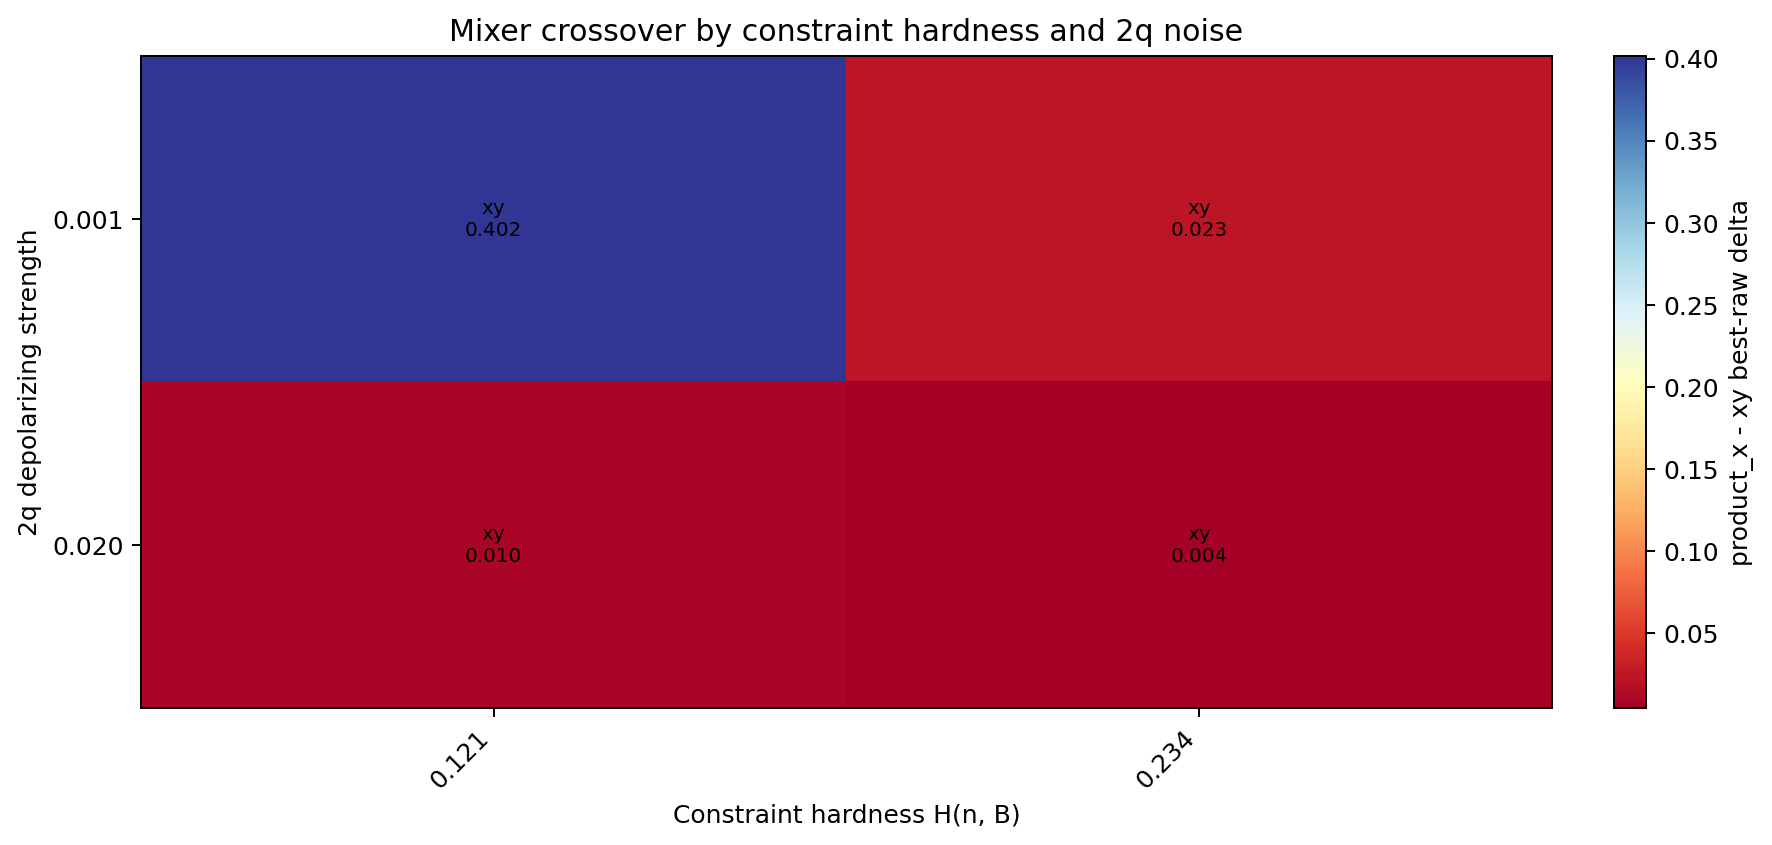
\includegraphics[width=0.82\linewidth]{figures/mixer_crossover.png}
\caption{Committed mixer-crossover heat map from \texttt{results/mixer\_dominance\_pilot\_v2/mixer\_crossover.png}. Each cell reports the mean delta \((\mathrm{product}\text{-}X - \mathrm{XY})\) in best raw objective, so positive values favor the \(\mathrm{XY}\) mixer. In the stored pilot, \(\mathrm{XY}\) wins in every tested \((H, p_{2q})\) cell, but the advantage shrinks noticeably at higher two-qubit depolarizing strength.}
\label{fig:mixer-crossover}
\end{figure}

The strongest individual mixer shift occurs in the \texttt{hard\_budget}, \(n=12\), low-noise context for Random Search, where the mean delta \((\mathrm{product}\text{-}X - \mathrm{XY})\) reaches \(2.9062\). This is not a universal statement about all methods or all regimes, but it is a strong indication that constraint-preserving dynamics matter most when the feasible sector is structurally difficult and the noise is still low enough for two-qubit gates to be useful.

\subsection{Hardware run: exact feasible energy is reachable, feasible occupancy is not}

The live IBM run is intentionally tiny, but it is scientifically valuable because it breaks the simulator-only ambiguity. The exact feasible energy for the three-asset, budget-one instance is \(-0.1661538\). Classical Markowitz returns that value exactly, as expected. The three quantum methods all discover the same best valid energy at least once; SPSA also matches it in the raw objective. On a score-only view, this looks encouraging.

The richer metrics show a harder reality. Table~\ref{tab:live-ibm} reports the live-hardware summaries. Random Search reaches the exact feasible energy with valid ratio \(0.640625\), SPSA with \(0.5625\), and BO with \(0.78125\). The dominant violations are ``off by one'' budget misses: Random Search produces 22 such shots out of 64, SPSA 25, and BO 14. Thus the \(\mathrm{XY}\) mixer preserves feasibility in the \emph{ideal} unitary model, but not under real hardware noise.

\begin{table}[H]
\centering
\caption{Live IBM run on \texttt{ibm\_fez} from \texttt{results/live\_ibm\_open\_2026\_04\_19/live\_run.json}. The transpiled circuit had depth \(120\), size \(166\), 31 two-qubit gates, and zero SWAPs for all quantum methods.}
\label{tab:live-ibm}
\begin{tabular}{l S[table-format=-1.4] S[table-format=-1.4] S[table-format=1.6] S[table-format=2.3] l}
\toprule
Method & {Best raw} & {Best valid} & {Valid ratio} & {Billed seconds} & {Violation counts} \\
\midrule
Classical Markowitz & -0.1662 & -0.1662 & 1.000000 & 0.000 & --- \\
Random Search & -0.1518 & -0.1662 & 0.640625 & 8.899 & \(\{0:41,1:22,2:1\}\) \\
SPSA & -0.1662 & -0.1662 & 0.562500 & 15.345 & \(\{0:36,1:25,2:3\}\) \\
Bayesian Optimization & -0.1458 & -0.1662 & 0.781250 & 7.061 & \(\{0:50,1:14\}\) \\
\bottomrule
\end{tabular}
\end{table}

Three points emerge from Table~\ref{tab:live-ibm}. First, best valid energy alone is too weak a live-hardware metric because all quantum methods eventually touch the exact feasible solution on this tiny instance. Second, valid ratio is much more revealing: the hardware repeatedly samples infeasible states, most often with budget violation \(1\). Third, BO has the best valid ratio and the lowest billed time among the quantum methods in this single-shot experiment, but its best raw objective is worse than Random Search and SPSA. This illustrates why the repository stores both raw and valid metrics: on hardware, the scientific question is often not ``which scalar won?'' but rather ``what kind of error pattern produced the scalar?''

\subsection{Representative figures}

Figure~\ref{fig:suite-dashboard} reproduces the committed suite dashboard and visually confirms the dominance of the classical baseline in the broad aggregate. Figure~\ref{fig:live-dashboard} shows the live-IBM dashboard. Together they illustrate the manuscript's central methodological claim: a meaningful benchmark must preserve the optimization trajectory, feasibility, and variance information, not just a terminal objective.

\begin{figure}[H]
\centering
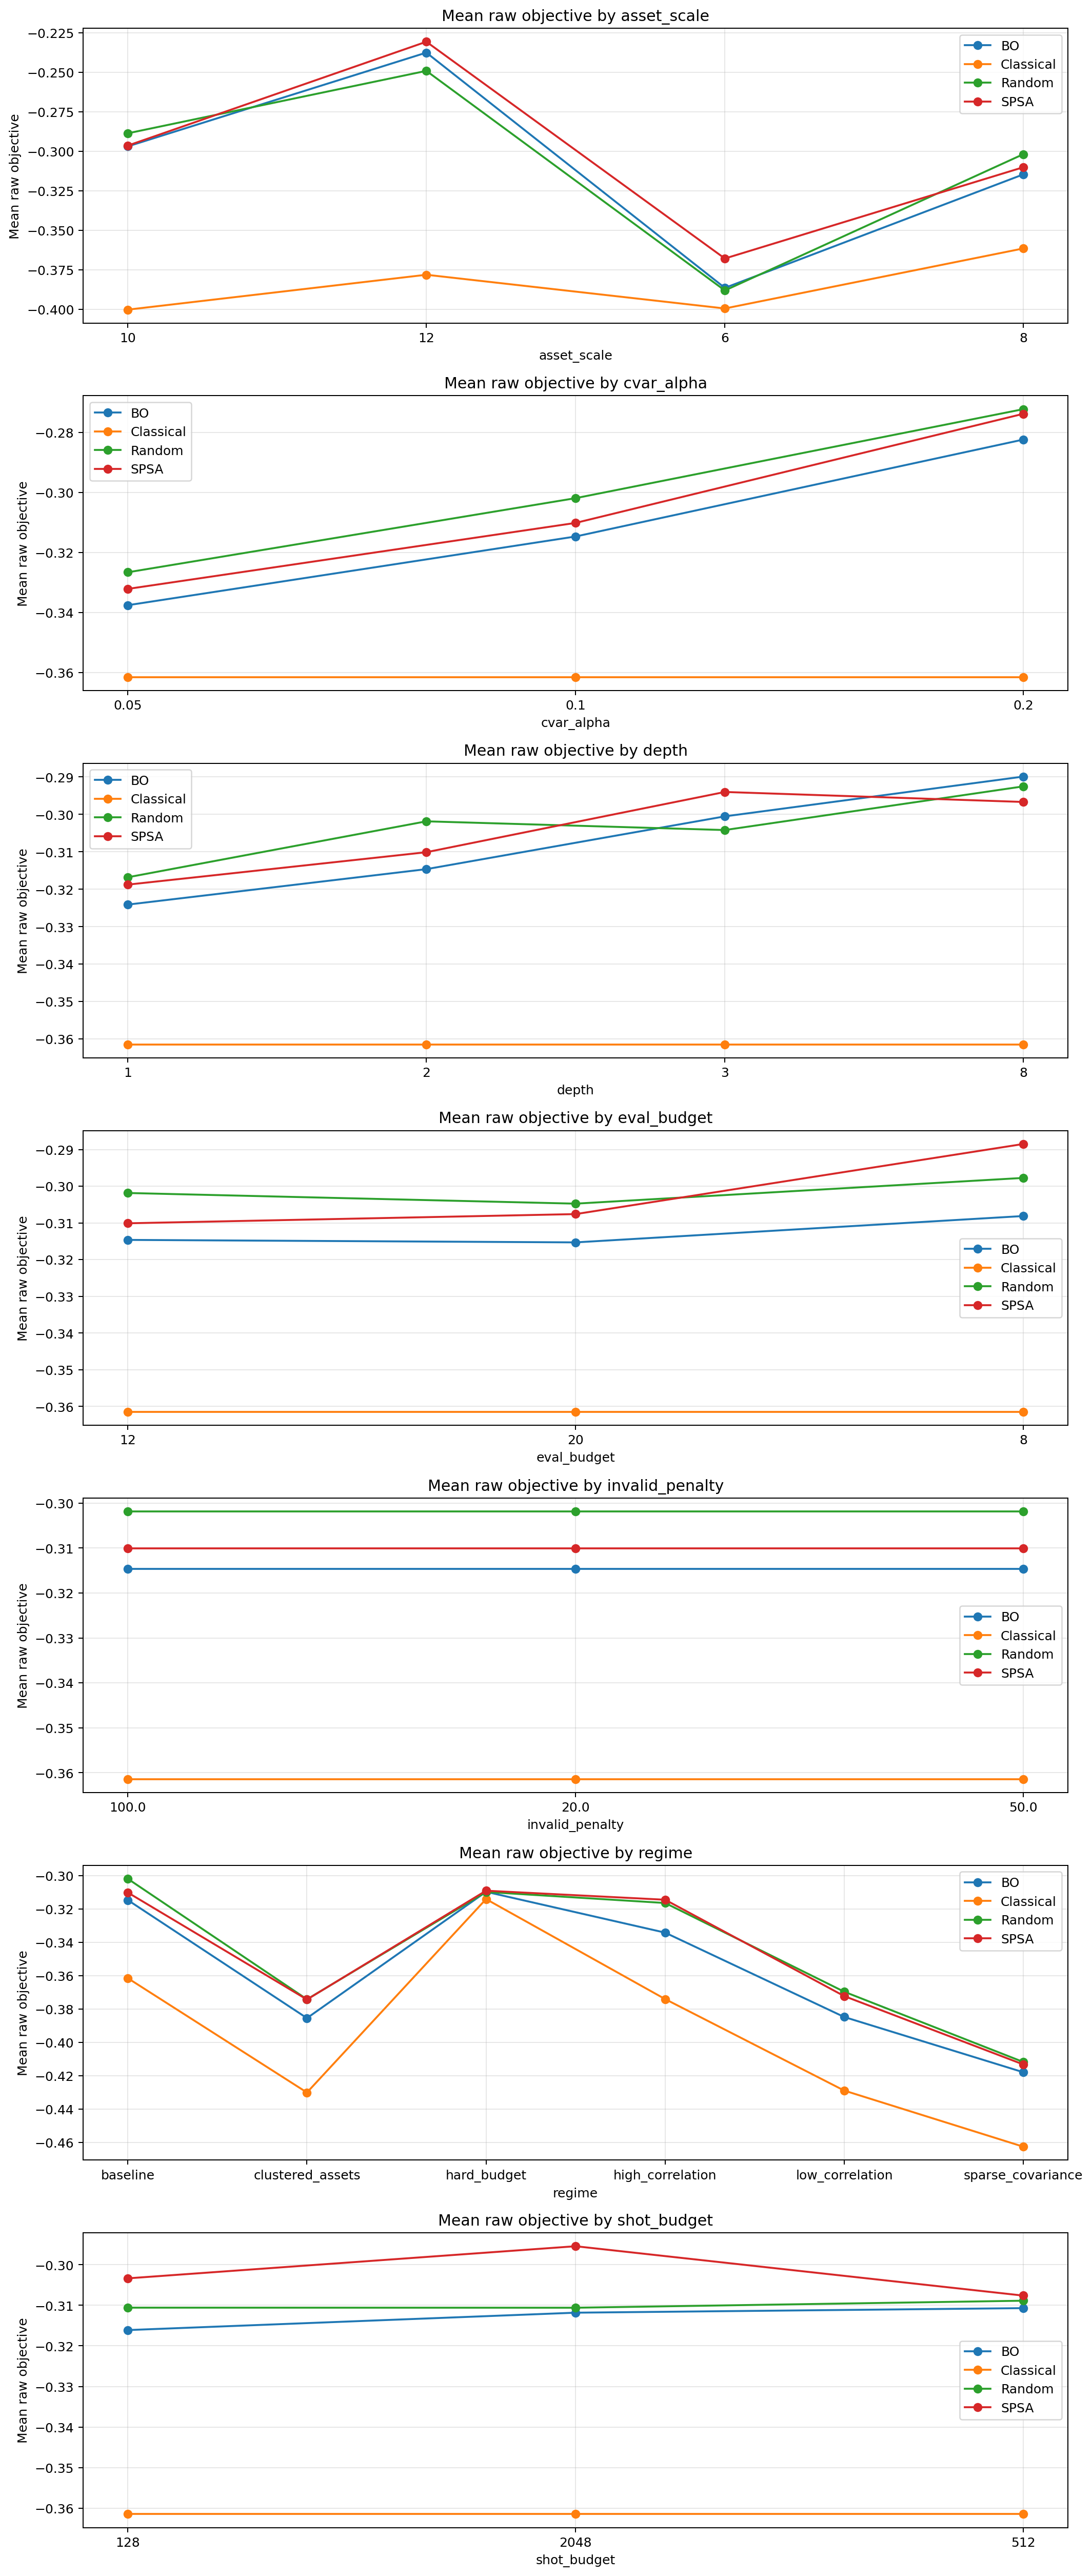
\includegraphics[width=\linewidth]{figures/multi_regime_suite_dashboard.png}
\caption{Committed dashboard from \texttt{results/multi\_regime\_suite/suite\_dashboard.png}. Across the stored contexts, the classical baseline remains visually separated from the quantum methods on mean best raw objective, while quantum win-rate differences are limited.}
\label{fig:suite-dashboard}
\end{figure}

\begin{figure}[H]
\centering
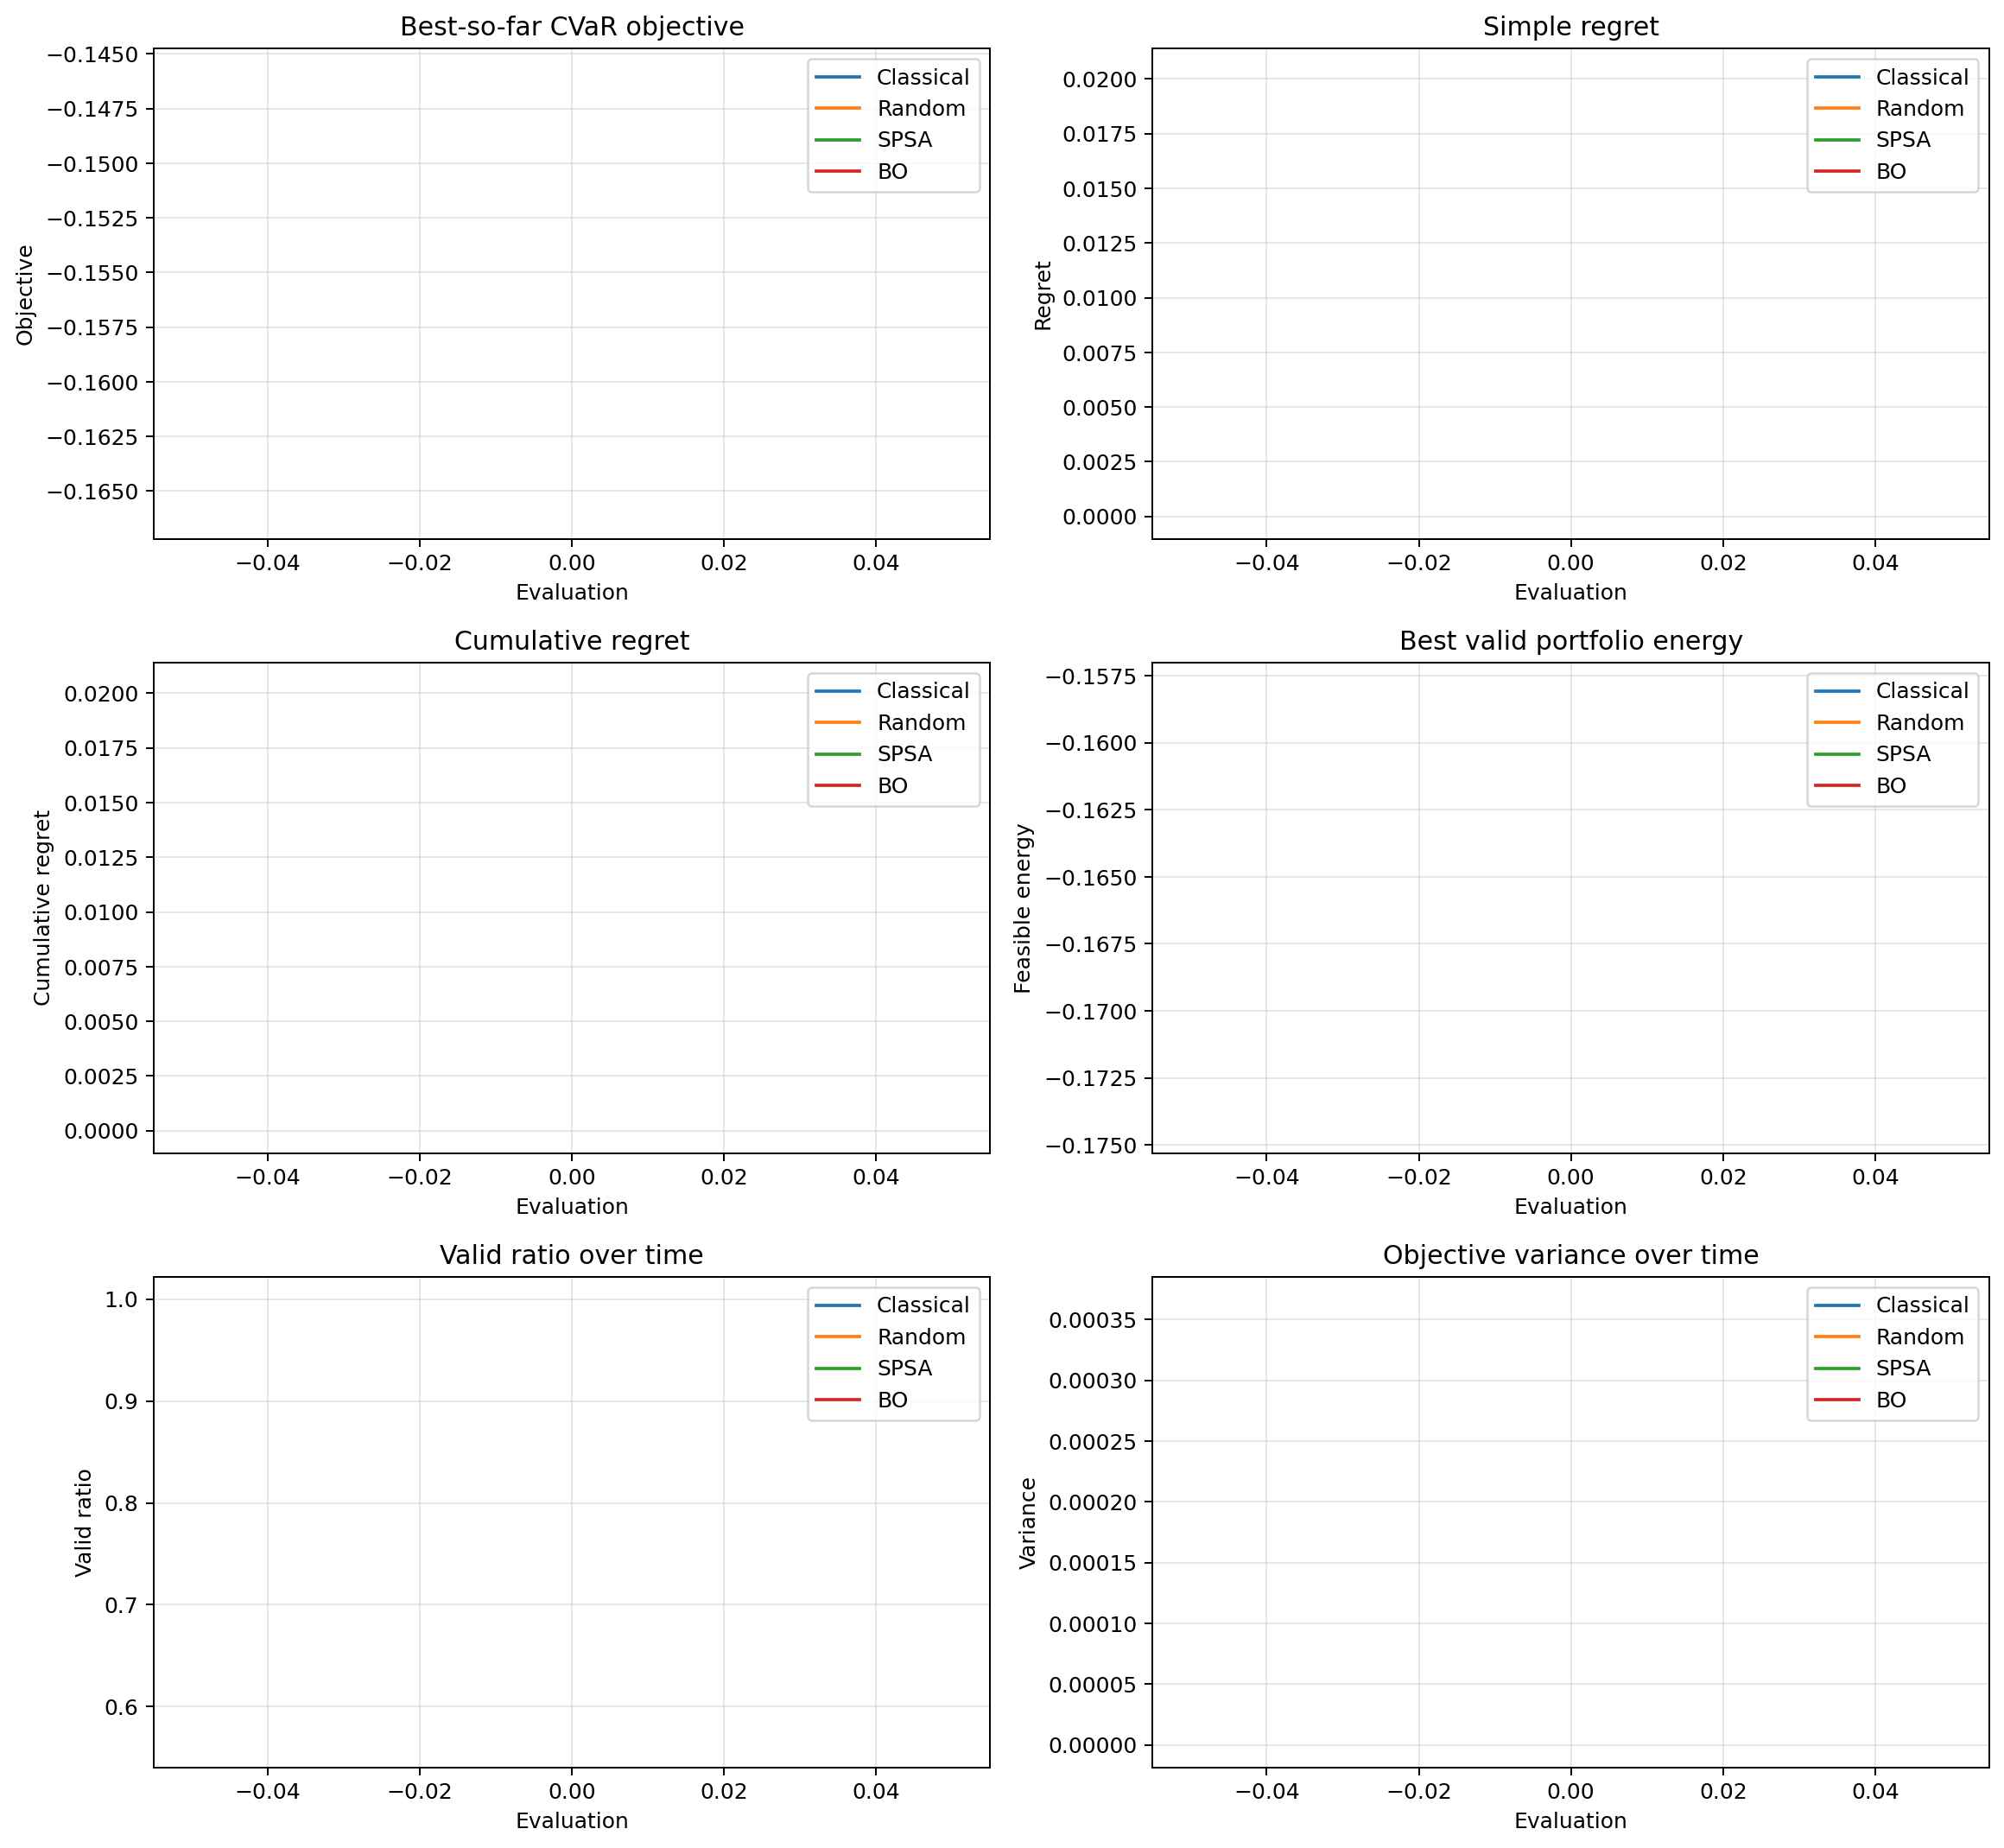
\includegraphics[width=0.92\linewidth]{figures/live_ibm_open_run.png}
\caption{Committed live-run dashboard from \texttt{results/live\_ibm\_open\_2026\_04\_19/live\_run.png}. The dashboard makes the disparity between best valid energy and feasible occupancy visually apparent.}
\label{fig:live-dashboard}
\end{figure}

\section{Discussion}\label{sec:discussion}

\subsection{What the results do and do not show}

The repository now supports a clean scientific claim, but it is more modest than a typical quantum-optimization sales pitch. The committed broad-suite evidence does \emph{not} show that BO justifies its hybrid-loop cost relative to simpler quantum optimizers. It does \emph{not} show that increasing QAOA depth helps under the tested budget and noise model. It does \emph{not} show that the quantum methods challenge, let alone exceed, the classical Markowitz baseline on the studied instances. Those null results are not failures of the manuscript; they are the main result.

At the same time, the evidence does show something scientifically useful. Constraint-preserving mixer design matters. The \(\mathrm{XY}\) mixer is consistently better than the penalty-based \(\mathrm{product}\text{-}X\) alternative in the clean pilot, and its advantage is largest in the structurally harder and cleaner parts of the tested space. This is a meaningful result because it isolates one architectural choice that changes the character of the search landscape itself. The stronger universal claim that ``the mixer is the algorithm'' is not yet supported by the pilot's variance decomposition, but the narrower statement that \(\mathrm{XY}\) is usually the better quantum mixer in the tested settings is supported.

\subsection{Why the classical baseline wins}

There are at least four mutually compatible reasons the classical baseline dominates the broad suite.
\begin{enumerate}[leftmargin=1.5em]
\item The tested instances are still small enough that exact or near-exact classical treatment remains easy.
\item The proxy-noise model and limited evaluation budgets restrict the extent to which QAOA can exploit additional expressivity.
\item The broad suite's shot and queue accounting penalizes quantum iterations far more than classical solves.
\item The Markowitz objective is structurally favorable to classical continuous relaxation and rounding, especially when cardinality is moderate.
\end{enumerate}

None of these explanations is embarrassing. On the contrary, they are precisely the kinds of boundary conditions that a serious characterisation study should surface. A realistic thesis in 2026 should not try to erase the fact that small portfolio QUBOs are classically tractable.

\subsection{Constraint preservation versus hardware cost}

The \(\mathrm{XY}\) mixer presents a classic NISQ trade-off. Theoretically, it preserves the budget subspace exactly, which is algorithmically attractive. Practically, it requires two-qubit entangling operations and therefore amplifies sensitivity to calibration error, decoherence, and routing. The committed pilot suggests that under the tested noise levels the algorithmic gain still dominates, but the margin shrinks at higher two-qubit noise. The live-IBM run reinforces the physical side of this story: even when the compiled circuit requires no SWAPs, the hardware still leaks population out of the feasible subspace. Thus the repository's most important mixer lesson is not that \(\mathrm{XY}\) solves the constraint problem outright, but that it moves the burden from the objective landscape into the hardware fidelity budget.

\subsection{Barren plateaus and missing diagnostics}

The present code base and manuscript discuss barren plateaus but do not yet produce a committed gradient-variance sweep over \(n\) and \(p\). That omission matters because the depth degradation observed in Table~\ref{tab:scale-depth} is consistent with either optimizer budget exhaustion or trainability loss. The correct interpretation is therefore conditional: the committed results are compatible with emerging trainability problems, especially under noise, but they do not yet isolate that mechanism experimentally \cite{mcclean2018barren,wang2021noisebarren}. A full thesis version should add the planned gradient-variance study rather than implying that the current evidence already proves one mechanism.

\subsection{Metric design lessons}

One of the clearest design lessons of the repository is that scalar summaries are treacherous. Feasible-hit rate saturates in the broad suite and therefore conceals differences in how well methods actually respect the budget. Best valid energy can look perfect on hardware even when nearly half the shots are infeasible. Raw objective can favor a method that simply exploits the penalty landscape rather than finding high-quality feasible portfolios. This is why the trace stores valid ratios, budget-violation histograms, Sharpe ratios, ZNE correction magnitudes, regret-area summaries, and shots-to-first-feasible. The committed results already vindicate this richer trace design: without it, the live-hardware run would look far more impressive than it actually is.

\subsection{Limitations}

The study has several explicit limitations.
\begin{itemize}[leftmargin=1.5em]
\item The broad precomputed suite uses a fast-simulator noise proxy rather than full backend calibration data.
\item The stored broad-suite aggregated artifact does not preserve full pairwise significance matrices, only the reported comparison against Random Search.
\item Real financial data are not yet included in the committed experiments; the study is synthetic by design.
\item The exact-reference logic is limited to \(n \leq 14\), which is scientifically appropriate for the current scale but not a substitute for larger-scale bounds.
\item The live hardware study is only a tiny open-access run and should not be overinterpreted.
\end{itemize}

These are genuine limitations, but they do not invalidate the manuscript's present claims because those claims are intentionally scoped to what the repository demonstrably supports.

\section{Future Work}\label{sec:future}

The strongest next steps are not cosmetic; they sharpen the scientific question.

First, the repository should commit a full constraint-hardness sweep using Eq.~\eqref{eq:hardness} as an explicit study axis. The hard-budget anomaly in Table~\ref{tab:regime-results} strongly suggests that feasible-subspace geometry modulates optimizer effectiveness. A dedicated study over \(B/n\) would test that directly.

Second, the broad suite should be augmented with a shot-allocation frontier at fixed total shot budget. The current artifact sweeps shots and evaluation budgets independently, but the practically relevant cloud-computing question is often how to allocate a fixed total number of circuit executions between noisier-but-more-numerous evaluations and cleaner-but-fewer evaluations.

Third, the planned barren-plateau and gradient-variance diagnostics should be committed. The current implementation already retains much of the per-evaluation structure needed to support that analysis, and the depth degradation in the broad suite makes the question timely.

Fourth, the mixer analysis should be extended into a true \((H,p_{2q})\) crossover study at larger scale and with live backend calibrations. The clean pilot suggests that such a crossover exists in principle, but the present grid is too small to estimate its location precisely.

Fifth, the classical baseline should be expanded into a richer financial evaluation protocol, including historical data, out-of-sample evaluation, and explicit portfolio-quality metrics beyond QUBO energy. The code already records Sharpe ratios for best valid portfolios; those should become first-class reporting outputs in future committed studies.

Finally, the warm-start hooks already present in the code should be used for a transfer study. Recent literature on warm-started QAOA and \(\mathrm{XY}\)-mixer geometry suggests that angle concentration and cross-instance transfer are plausible and potentially important \cite{egger2021warm,kordonowy2026lie,mancilla2026portfolio}.

\section{Conclusion}\label{sec:conclusion}

This manuscript has presented a rigorous, repository-grounded characterisation of constrained QAOA portfolio optimization. The project contribution is not an isolated demonstration circuit or an unqualified benchmark claim; it is a reproducible scientific instrument that connects QUBO construction, feasible-subspace geometry, constrained and unconstrained mixers, classical optimizer choice, backend-aware execution, and runtime-cost accounting in one auditable workflow.

The empirical findings are mixed in exactly the way credible near-term quantum research should expect. The broad suite shows that a classical Markowitz baseline dominates every stored study slice and that no quantum outer-loop optimizer in the stored artifact achieves statistically significant superiority over Random Search. The mixer pilot shows that the \(\mathrm{XY}\) mixer is usually the stronger quantum architecture, especially in harder and cleaner settings, but does not support the stronger blanket claim that mixer choice dominates optimizer choice. The live IBM run shows that exact feasible solutions can be reached on real hardware for a tiny instance, but that feasible occupancy degrades substantially under realistic noise even when the ansatz is constraint preserving in the ideal model.

The principal scientific value of the repository is therefore methodological clarity. It identifies where strong claims fail, where narrower claims survive, and what instrumentation is required to tell the difference. For a field in which impressive scalar outcomes are often reported without enough context, that is a meaningful contribution in its own right.

\bibliographystyle{IEEEtran}
\bibliography{references}

\appendix

\section{Notation Table}\label{app:notation}

\begin{longtable}{p{0.18\linewidth}p{0.74\linewidth}}
\caption{Notation used throughout the manuscript.}\label{tab:notation}\\
\toprule
Symbol & Meaning \\
\midrule
\endfirsthead
\toprule
Symbol & Meaning \\
\midrule
\endhead
\(n\) & Number of assets, equal to the number of qubits in the current binary encoding. \\
\(B\) & Portfolio cardinality budget. \\
\(x \in \{0,1\}^n\) & Binary portfolio-selection vector. \\
\(\mu \in \mathbb{R}^n\) & Expected-return vector. \\
\(\Sigma \in \mathbb{R}^{n\times n}\) & Symmetric covariance estimate. \\
\(q\) & Risk-aversion coefficient. \\
\(P\) & Budget-penalty coefficient used in the penalized QUBO. \\
\(Q\) & Penalized QUBO matrix. \\
\(\mathcal{H}\) & Full \(n\)-qubit Hilbert space \((\mathbb{C}^2)^{\otimes n}\). \\
\(\mathcal{H}_B\) & Hamming-weight-\(B\) feasible subspace. \\
\(H(n,B)\) & Feasible-subspace fraction \(\binom{n}{B}/2^n\). \\
\(H_C\) & Problem Hamiltonian derived from the penalized QUBO. \\
\(H_M^{(X)}\) & Product-\(X\) mixer Hamiltonian. \\
\(H_M^{(\mathrm{XY})}\) & Constraint-preserving \(\mathrm{XY}\) mixer Hamiltonian. \\
\(\bm{\gamma},\bm{\beta}\) & QAOA phase-separator and mixer angles. \\
\(\rho_{\bm{\gamma},\bm{\beta}}\) & Noisy density operator after circuit execution. \\
\(\alpha\) & CVaR tail fraction. \\
\(\widehat{\sigma}_{\mathrm{tail}}^2\) & Lower-tail energy variance. \\
\(\widehat{\sigma}_{\mathrm{shot}}^2\) & Shot-noise proxy used by the repository. \\
\bottomrule
\end{longtable}

\section{Additional Tables}\label{app:tables}

\begin{table}[H]
\centering
\caption{Mixer-versus-optimizer balance for the clean pilot. Positive mixer effect means the mean \(\mathrm{XY}\) advantage over \(\mathrm{product}\text{-}X\) within the context; optimizer effect is the spread among methods within the same context.}
\label{tab:mixer-balance}
\begin{tabular}{l c c l S[table-format=1.4] S[table-format=1.4] S[table-format=1.6]}
\toprule
Regime & \(n\) & \(p_{2q}\) & Dominant factor & {Mixer effect} & {Optimizer effect} & {Hardness} \\
\midrule
baseline & 6 & 0.001 & mixer & 0.0432 & 0.0395 & 0.234375 \\
baseline & 6 & 0.020 & optimizer & 0.0081 & 0.0433 & 0.234375 \\
baseline & 12 & 0.001 & optimizer & 0.0725 & 0.1292 & 0.120850 \\
baseline & 12 & 0.020 & optimizer & 0.0170 & 0.1781 & 0.120850 \\
hard\_budget & 6 & 0.001 & mixer & 0.0029 & 0.0023 & 0.234375 \\
hard\_budget & 6 & 0.020 & optimizer & 0.0007 & 0.0033 & 0.234375 \\
hard\_budget & 12 & 0.001 & optimizer & 0.7310 & 1.4604 & 0.120850 \\
hard\_budget & 12 & 0.020 & optimizer & 0.0031 & 0.0250 & 0.120850 \\
\bottomrule
\end{tabular}
\end{table}

\begin{table}[H]
\centering
\caption{Selected broad-suite shot-budget and CVaR sweeps.}
\label{tab:shot-cvar}
\begin{tabular}{l c l S[table-format=-1.4]}
\toprule
Study & Value & Best quantum method & {Best quantum mean raw} \\
\midrule
shot budget & 128 & Bayesian Optimization & -0.3161 \\
shot budget & 512 & Bayesian Optimization & -0.3107 \\
shot budget & 2048 & Bayesian Optimization & -0.3118 \\
\midrule
CVaR \(\alpha\) & 0.05 & Bayesian Optimization & -0.3375 \\
CVaR \(\alpha\) & 0.10 & Bayesian Optimization & -0.3146 \\
CVaR \(\alpha\) & 0.20 & Bayesian Optimization & -0.2823 \\
\bottomrule
\end{tabular}
\end{table}

\section{Environment and Reproducibility Notes}\label{app:environment}

The repository's declared environment boundary is:
\begin{itemize}[leftmargin=1.5em]
\item Python \(\geq\) 3.10.
\item Core dependencies: NumPy \(\geq 1.26\), SciPy \(\geq 1.12\), scikit-learn \(\geq 1.5\), Matplotlib \(\geq 3.8\), PyYAML \(\geq 6.0\).
\item Optional BO extras: PyTorch \(\geq 2.2\), BoTorch \(\geq 0.16\), GPyTorch \(\geq 1.14\).
\item Optional quantum extras: Qiskit \(\geq 2.3\), Qiskit Aer \(\geq 0.17\), Qiskit IBM Runtime \(\geq 0.46\).
\end{itemize}

The exact committed result files cited in the manuscript are:
\begin{itemize}[leftmargin=1.5em]
\item \texttt{results/multi\_regime\_suite/suite\_aggregated.csv}
\item \texttt{results/multi\_regime\_suite/suite\_report.md}
\item \texttt{results/multi\_regime\_suite/suite\_dashboard.png}
\item \texttt{results/mixer\_dominance\_pilot\_v2/mixer\_dominance\_summary.csv}
\item \texttt{results/mixer\_dominance\_pilot\_v2/mixer\_optimizer\_balance.csv}
\item \texttt{results/mixer\_dominance\_pilot\_v2/mixer\_variance\_summary.json}
\item \texttt{results/mixer\_dominance\_pilot\_v2/mixer\_crossover.png}
\item \texttt{results/live\_ibm\_open\_2026\_04\_19/live\_run.json}
\item \texttt{results/live\_ibm\_open\_2026\_04\_19/live\_run.png}
\end{itemize}

The manuscript is intentionally limited to claims supported by those committed artifacts. Where the current code base contains features not fully exercised in the committed broad suite, they are discussed as implementation capability rather than as empirical findings.

\section{Additional Code Listings}\label{app:listings}

\begin{lstlisting}[language=Python,caption={\texttt{SyntheticMarket.\_hard\_budget\_regime()} excerpt.},label={lst:market}]
def _hard_budget_regime(cfg: RunSpec, rng: np.random.Generator):
    n_assets = cfg.n_assets
    budget_fraction = cfg.budget / max(cfg.n_assets, 1)
    middle_pressure = 1.0 - abs(0.5 - budget_fraction) * 2.0
    base_return = rng.uniform(0.09, 0.12)
    edge = 0.0025 - 0.0010 * middle_pressure
    signal = np.concatenate([
        np.full(cfg.budget, edge, dtype=float),
        np.full(n_assets - cfg.budget, -edge, dtype=float),
    ])
    rng.shuffle(signal)
    mu = base_return + signal + 0.0015 * rng.standard_normal(n_assets)
    common = rng.standard_normal((n_assets, 2))
    sigma = (0.010 + 0.006 * middle_pressure) * (common @ common.T)
    sigma /= max(float(np.mean(np.diag(sigma))), 1e-6)
    sigma *= 0.012
    sigma += (0.0015 + 0.0015 * middle_pressure) * np.eye(n_assets)
    return mu, sigma
\end{lstlisting}

\begin{lstlisting}[language=Python,caption={Constraint-hardness and spectral-profile excerpt.},label={lst:landscape-note}]
def constraint_hardness(n_assets: int, budget: int) -> float:
    return feasibility_subspace_size(n_assets, budget) / float(2**n_assets)

def profile_instance(instance: PortfolioQUBO) -> QUBOSpectralProfile:
    base = np.asarray(instance.base_matrix, dtype=float)
    eigenvalues = np.linalg.eigvalsh(base)
    ...
    states = np.arange(1 << n_assets, dtype=np.uint64)
    bits = ((states[:, None] >> np.arange(n_assets, dtype=np.uint64)) & 1).astype(float)
    cardinalities = bits.sum(axis=1)
    energies = np.einsum("bi,ij,bj->b", bits, instance.base_matrix, bits, optimize=True)
    feasible = cardinalities == instance.budget
    infeasible = ~feasible
    ...
\end{lstlisting}

\begin{lstlisting}[language=Python,caption={Optimizer excerpts: BO warm start and SPSA calibration.},label={lst:optimizers}]
if self.cfg.warm_start_params:
    warm_start = project_params(
        np.asarray(self.cfg.warm_start_params, dtype=float),
        self.bounds,
        periodic_wrap=self.cfg.periodic_parameter_wrap,
    )
    self.init_design[0] = warm_start

...

ghat = (stats_plus.objective - stats_minus.objective) / (2.0 * ck * delta)
if k == 1:
    grad_norm = float(np.linalg.norm(ghat))
    if grad_norm > 1e-8:
        a = 0.1 * float(np.mean(bounds[1] - bounds[0])) / grad_norm
ak = a / ((k + A) ** 0.602)
x = project_params(x - ak * ghat, bounds, periodic_wrap=cfg.periodic_parameter_wrap)
\end{lstlisting}

\begin{lstlisting}[language=Python,caption={\texttt{run\_benchmark()} orchestration excerpt.},label={lst:pipeline}]
mu, sigma = SyntheticMarket.build(cfg, rng)
instance = QuboFactory.build(mu, sigma, cfg)
spectral_profile = profile_instance(instance)
executor = build_executor(instance, cfg)
bounds = make_bounds(cfg)

classical_trace = run_classical_markowitz(instance, cfg)
random_trace = run_random_search(executor, cfg, bounds, rng)
spsa_trace = run_spsa_search(executor, cfg, bounds, rng)
bo_trace = run_bayesian_search(executor, cfg, bounds, rng, progress=...)

traces = {
    "classical_markowitz": classical_trace,
    "random": random_trace,
    "spsa": spsa_trace,
    "bayesian_optimization": bo_trace,
}
plot_results(traces, prefix)
payload = save_summary(cfg, instance, traces, prefix, spectral_profile=spectral_profile)
\end{lstlisting}

\end{document}
